%% IEEE Conference Paper
%% Condensed from: Hybrid Event-Driven Spoofing Detection in Energy-Constrained WSNs
%% Target venue: IEEE conference (GLOBECOM / INFOCOM / SECON / ICC)
%% Target length: 6 pages

\documentclass[conference]{IEEEtran}
\IEEEoverridecommandlockouts
% The preceding line is only needed to identify funding in the first footnote. If that is unneeded, please comment it out.

\usepackage{amsmath,amssymb,amsfonts}
\usepackage{lmodern}          % Vector font rendering for crisp PDF output
\usepackage{graphicx}
\usepackage{textcomp}
\usepackage{url}
\usepackage[hidelinks]{hyperref}

\def\BibTeX{{\rm B\kern-.05em{\sc i\kern-.025em b}\kern-.08em
    T\kern-.1667em\lower.7ex\hbox{E}\kern-.125emX}}

\providecommand{\toprule}{\hline\hline}
\providecommand{\midrule}{\hline}
\providecommand{\bottomrule}{\hline\hline}

% Compact float & equation spacing for strict conference page budget
\setlength{\textfloatsep}{4pt plus 2pt minus 2pt}
\setlength{\floatsep}{4pt plus 2pt minus 2pt}
\setlength{\intextsep}{4pt plus 2pt minus 2pt}
\setlength{\dbltextfloatsep}{4pt plus 2pt minus 2pt}
\setlength{\abovecaptionskip}{2pt}
\setlength{\belowcaptionskip}{-4pt}
\setlength{\abovedisplayskip}{2pt plus 1pt minus 1pt}
\setlength{\belowdisplayskip}{2pt plus 1pt minus 1pt}

\hyphenation{physio-ener-getic micro-con-troller micro-con-trollers multi-path multi-attribute}

\begin{document}

\title{Hybrid Event Driven Spoofing Detection in Energy Constrained Wireless Sensor Networks}

\author{
\IEEEauthorblockN{Prashanth K}
\IEEEauthorblockA{\textit{Department of Master of Computer Applications} \\
\textit{RV College of Engineering (Affiliated to VTU, Belagavi)}\\
Bengaluru, India \\
prashanthk@rvce.edu.in}
\and
\IEEEauthorblockN{Dr. Usha J}
\IEEEauthorblockA{\textit{Department of Master of Computer Applications} \\
\textit{RV College of Engineering (Affiliated to VTU, Belagavi)}\\
Bengaluru, India \\
ushaj@rvce.edu.in}
}

\maketitle

% ----------------------------------------------------------------
\begin{abstract}
Resource-constrained Wireless Sensor Networks (WSNs) deployed in industrial monitoring remain vulnerable to identity spoofing attacks due to shared wireless channels and unencrypted MAC headers. While continuous cryptographic verification offers origin authentication, signature verification consumes an unsustainable 90 mJ per packet on 16-bit microcontrollers, leading to rapid Cluster Head battery exhaustion within 3 days. Conversely, lightweight Received Signal Strength Indicator (RSSI) physical-layer filters consume minimal energy but suffer from false positive rates exceeding 12\% under severe multipath fading. We present the Hybrid Event-Driven Spoofing Detection (HEDSD) framework to reconcile this fundamental energy-security trade-off. HEDSD extracts a four-dimensional behavioral feature vector combining spatial RSSI statistics, packet inter-arrival rate, and Cluster Head battery depletion rate mapped into normalized anomaly indicators and a composite score. A three-tier battery-adaptive state machine dynamically scales monitoring intensity, invoking cryptographic audits only when anomaly indicators cross dynamic conjunctive thresholds. Evaluated across extensive NS-3 discrete-event simulations and validated on a physical ESP32 testbed, HEDSD reduces per-packet evaluation energy by 99.4\% while achieving a detection recall of 98.2\%, an Area Under the ROC Curve of 0.998, a false positive rate of 0.03\%, and subsecond threat isolation latency (0.85 s). This extends projected Cluster Head battery operational lifetime under active attack from 3 to 397 days.
\end{abstract}

\begin{IEEEkeywords}
Wireless Sensor Networks, Spoofing Detection, Physical-Layer Security, Battery-Adaptive Security, Multi-Feature Anomaly Detection.
\end{IEEEkeywords}

% ================================================================
\section{Introduction}
\label{sec:intro}

Wireless Sensor Networks (WSNs) serve as the fundamental sensing backbone for modern Industrial Internet of Things (IIoT) applications, including automated smart power grids, oil pipeline monitoring, and industrial supervisory control and data acquisition (SCADA) systems~\cite{ref_iot_survey_01,ref_wsn_ind_02}. In these deployments, hundreds of battery-powered sensor motes continuously capture field telemetry and forward 128-byte data frames over low-power IEEE 802.15.4 wireless channels to designated Cluster Heads (CHs). However, because standard radio channels broadcast openly without mandatory per-packet cryptographic encapsulation, WSNs remain vulnerable to identity spoofing and frame injection attacks~\cite{ref_spoof_survey_07,ref_sybil_08}. An adversary can forge the unencrypted Media Access Control (MAC) address or node identifier of a legitimate sensor to inject malicious telemetry readings, alter cluster routing tables, mask equipment failures, or trigger false emergency shutdowns, making robust, real-time node authentication a critical security requirement.

Addressing identity spoofing under strict node hardware constraints reveals a fundamental energy-security dilemma in resource-limited sensor networks. Conventional defenses fall into two inadequate paradigms. Cryptographic authentication schemes, such as the Elliptic Curve Digital Signature Algorithm (ECDSA NIST P-256), guarantee origin authenticity but consume an unsustainable $90.0\,\text{mJ}$ per signature verification on 16-bit MSP430 microcontrollers~\cite{ref_mcu_energy_12,ref_ecc_wsn_10}. Under active packet transmission, executing continuous signature verification exhausts standard Cluster Head battery reserves ($50.0\,\text{kJ}$) within $3.0\,\text{days}$, creating an energy-depletion Denial-of-Service (DoS) vulnerability. Conversely, lightweight physical-layer authentication techniques exploit Received Signal Strength Indicator (RSSI) profiles at low energy cost ($<5.0\,\mu\text{J}/\text{pkt}$)~\cite{ref_yang_rssi_20}, but incur false positive rates exceeding $12\%$ under log-normal shadowing ($\sigma_\text{dB}=10\,\text{dB}$) and multipath fading~\cite{ref_rssi_fading_16}. Furthermore, recent machine learning (ML) classifiers achieve high accuracy ($94\%\text{--}98\%$) but demand $0.35$--$2.50\,\text{mJ}/\text{pkt}$ and over $10\,\text{kB}$ RAM, exceeding commodity microcontroller capabilities~\cite{ref_jsen_svm_2022,ref_iotj_fedtrust_2024}.

HEDSD addresses these dual constraints by fusing spatial physical-layer screening, packet inter-arrival timing, and real-time receiver battery drain rate monitoring into a battery-adaptive decision architecture. Cryptographic audits are invoked selectively only when composite anomaly indicators cross dynamic conjunctive thresholds.

The remainder of this paper is organized as follows. Section~\ref{sec:model} establishes the system and threat models. Section~\ref{sec:method} presents the proposed HEDSD framework. Section~\ref{sec:eval} evaluates classification efficacy, energy efficiency, and testbed fidelity. Section~\ref{sec:discussion} discusses operational limitations, and Section~\ref{sec:conclusion} concludes the paper.

% ================================================================
\section{System Model and Threat Model}
\label{sec:model}

\subsection{System and Network Model}
The network topology comprises a clustered Wireless Sensor Network spanning a $1000\,\text{m} \times 1000\,\text{m}$ industrial field, containing $N_\text{total} = 401$ total nodes: $N_\text{CH} = 40$ Cluster Heads arranged in an $8 \times 5$ grid layout and $N_\text{leaf} = 361$ leaf sensor motes reporting to a central Base Station located at coordinates $(500, 500)\,\text{m}$~\cite{ref_ns3_official_36}. Leaf motes capture environmental telemetry and transmit 128-byte data frames over IEEE 802.15.4 channels with a nominal packet inter-arrival time of $2.0\,\text{s}$. Nodes are powered by non-rechargeable dual-AA alkaline batteries supplying an initial energy reserve of $21.6\,\text{kJ}$ ($3.0\,\text{V}$, $2000\,\text{mAh}$) for leaf motes and $50.0\,\text{kJ}$ for Cluster Heads.

\begin{figure}[htbp]
\centering
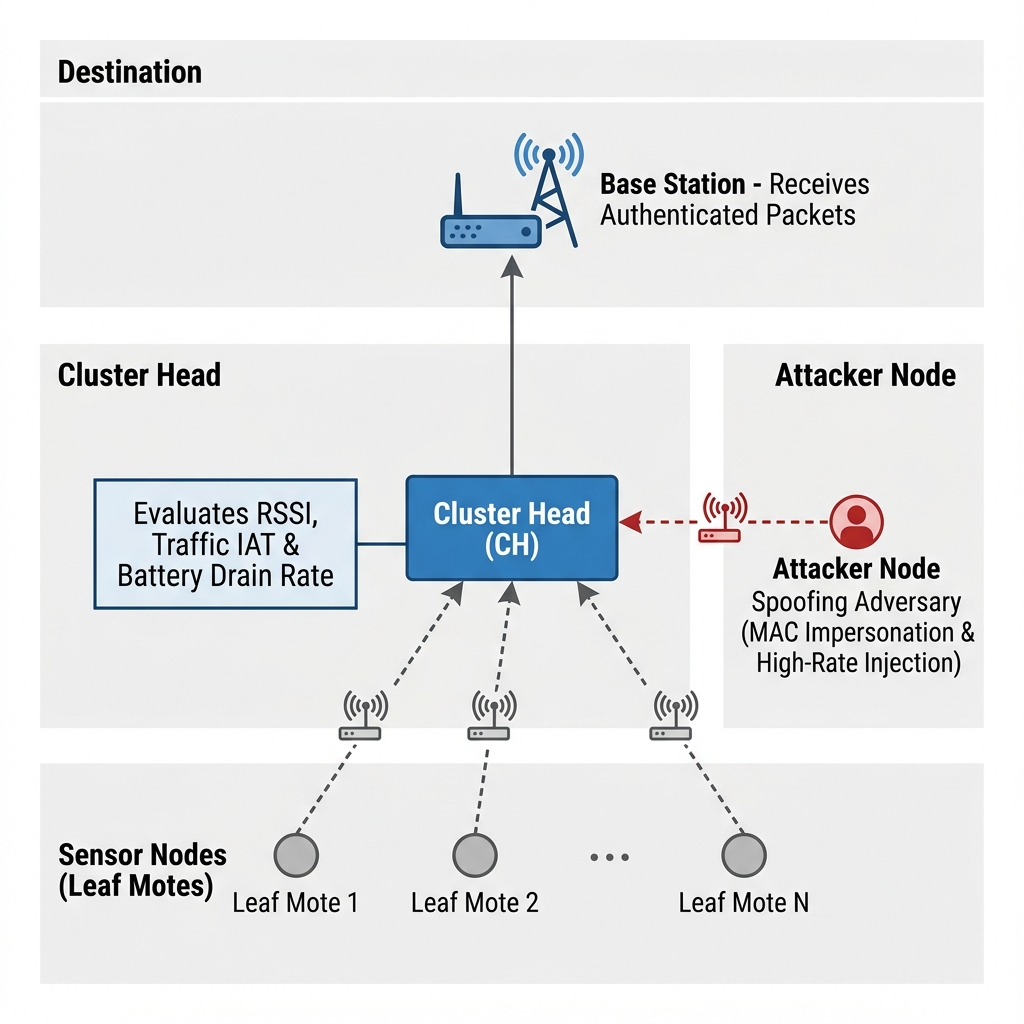
\includegraphics[width=0.88\columnwidth]{wsn_architecture_classical.png}
\caption{Clustered WSN deployment topology.}
\label{fig:architecture}
\end{figure}

To constrain identity spoofing attacks before malicious traffic propagates through the network backbone, HEDSD establishes Cluster Heads as localized physio-energetic checkpoints. As illustrated in Fig.~\ref{fig:architecture}, legitimate sensor motes capture environmental telemetry and transmit 128-byte data frames to their designated Cluster Head over wireless channels, while an active spoofing adversary attempts to inject forged packets by impersonating valid MAC addresses. Localizing anomaly detection to the Cluster Head prevents forged frames from traversing the multi-hop routing backbone to the Base Station, bounding physical attack propagation and saving core relay node energy.

Energy consumption for packet transmission and reception follows the first-order radio propagation model:
\begin{align}
E_\text{tx}(k,d) &= k E_\text{elec} + k\,\varepsilon_\text{amp}\,d^n \label{eq:etx} \\[2pt]
E_\text{rx}(k) &= k E_\text{elec} \label{eq:erx}
\end{align}
where $E_\text{elec} = 50\,\text{nJ/bit}$ is the transceiver circuit dissipation constant, $\varepsilon_\text{amp} = 100\,\text{pJ/bit/m}^n$ is the transmitter amplifier parameter specified relative to reference distance $d_0 = 1.0\,\text{m}$, $k = 1024\,\text{bits}$ is the frame length, and $n = 2.7$ represents the industrial path-loss exponent. The received signal strength for a mote at distance $d$ from the Cluster Head is modeled as:
\begin{equation}
\text{RSSI}(d) = P_\text{tx} - \text{PL}(d_0) - 10 \, n \log_{10}(d/d_0) + X_\sigma
\label{eq:pathloss}
\end{equation}
where $P_\text{tx} = 0\,\text{dBm}$ is the nominal transmit power, $\text{PL}(d_0) = 40.2\,\text{dB}$ is the reference path loss at $d_0 = 1.0\,\text{m}$, and $X_\sigma \sim \mathcal{N}(0, \sigma_\text{dB}^2)$ with $\sigma_\text{dB} = 10\,\text{dB}$ represents log-normal shadowing fading. Furthermore, the real-time Cluster Head battery energy drain rate $\dot{E}_i$ during packet evaluation is expressed as:
\begin{equation}
\dot{E}_i = \frac{dE_i}{dt} = \frac{E_\text{rx}(k) + E_\text{proc}(p_i)}{\Delta t_i}
\label{eq:battery_drain}
\end{equation}
where $E_\text{proc}(p_i)$ denotes the computational energy expended to process packet $p_i$ and $\Delta t_i$ is the inter-packet reception interval.

\subsection{Threat Model and Attacker Taxonomy}
We consider an active, resource-capable wireless adversary deploying up to $N_\text{attacker} = 108$ malicious attacker nodes across the $401$-node network ($D_\text{adv} = N_\text{attacker}/N_\text{leaf} \le 30\%$ node-level attacker density), where $N_\text{attacker} \subseteq N_\text{leaf}$ represents a compromised subset of the leaf node population. Attackers operate across three density regimes: low ($D_\text{adv}=5\%$, $N_\text{attacker}=18$), medium ($D_\text{adv}=15\%$, $N_\text{attacker}=54$), and high ($D_\text{adv}=30\%$, $N_\text{attacker}=108$), producing a net packet attack prevalence of $P_\text{attack} = 0.53\%$ ($5{,}938$ spoofed frames out of $1{,}120{,}555$ evaluated packets).

1) \textit{Adversary Capabilities and Limitations}: The adversary can eavesdrop on unencrypted IEEE 802.15.4 wireless channels, extract legitimate MAC addresses from telemetry headers, and dynamically alter transmission parameters, including transmit power $P_\text{tx}^{(\text{adv})}$, packet inter-arrival intervals $\text{IAT}_i$, and frame sequence numbers. However, the adversary cannot extract master cryptographic keys stored in secure Cluster Head hardware or alter physical radio propagation physics ($n = 2.7, \sigma_\text{dB} = 10\,\text{dB}$). Crucially, the adversary cannot suppress the physical energy required by receiving Cluster Head circuitry to demodulate, buffer, and process incoming frames \eqref{eq:battery_drain}.

2) \textit{Attacker Behavioral Models}: Attackers execute spoofing vectors quantified by spatial signal deviation $\Delta\text{RSSI}_i$ and packet injection rate acceleration $\lambda_\text{IAT}^{(i)}$:
\begin{align}
\Delta\text{RSSI}_i &= |\text{RSSI}_\text{obs}^{(i)} - \text{RSSI}_\text{exp}^{(i)}| > \delta_\text{spatial} \label{eq:mac_spoof} \\[4pt]
\lambda_\text{IAT}^{(i)} &= \frac{1}{\text{IAT}_i} > \lambda_\text{nominal} \label{eq:rate_injection}
\end{align}
\begin{itemize}
    \item \textbf{Displaced Identity Impersonation}: A rogue node positioned at spatial offset $d > 5.0\,\text{m}$ forges the MAC address of a legitimate victim sensor, producing spatial signal deviation $\Delta\text{RSSI}_i > \delta_\text{spatial}$ \eqref{eq:mac_spoof}.
    \item \textbf{High-Rate Energy-Depletion Flooding}: Attackers reduce nominal packet intervals from $2.0\,\text{s}$ to $0.5\,\text{s}$ ($\lambda_\text{IAT}^{(i)} > 0.5\,\text{s}^{-1}$) \eqref{eq:rate_injection}, flooding the Cluster Head to induce routing queue congestion and force high-power cryptographic evaluations ($90.0\,\text{mJ/pkt}$).
    \item \textbf{Colluding Multi-Node Attackers}: Synchronized malicious motes ($N_\text{attacker} \le 108$) coordinate frame injection across adjacent cluster grid cells ($N_\text{CH}=40$), interleaving bursts to evade single-node temporal rate thresholds.
    \item \textbf{Adaptive Power-Control Evasion}: An adversary at distance $d_\text{adv} > d_\text{target}$ dynamically scales transmit power $P_\text{tx}^{(\text{adv})} = P_\text{tx}^{(\text{target})} + 10n \log_{10}(d_\text{adv}/d_\text{target})$ to force spatial deviation $\Delta\text{RSSI}_i \to 0\,\text{dBm}$, seeking to bypass Tier-1 RSSI screening.
\end{itemize}

3) \textit{Industrial SCADA Threat Scenarios}: Attackers exploit these behavioral models to execute two industrial SCADA attack vectors: (i)~*False Telemetry Injection*, where forged sensor frames inject corrupted pressure or flow telemetry to trigger false emergency plant shutdowns or mask real equipment failures; and (ii)~*Energy-Depletion Denial-of-Service (E-DoS)*, where high-rate frame bursts force Cluster Heads into sustained high-current signature verification states ($185.2\,\text{mA}$ peak current), accelerating battery capacity loss via internal resistance heating ($I^2 R_\text{int}$).

% ================================================================
\section{Proposed HEDSD Framework}
\label{sec:method}

\subsection{Multi-Feature Anomaly Engine}
For each incoming telemetry frame $p_k$ received at Cluster Head $\text{CH}_j$ from a claimed node $N_i$, HEDSD extracts a composite four-dimensional behavioral feature vector:
\begin{equation}
\mathbf{F}_i(t) = \left[ \mu_{\text{RSSI}}^{(i)}, \, \sigma_{\text{RSSI}}^{(i)}, \, \lambda_{\text{IAT}}^{(i)}, \, \dot{E}_i \right]^T
\label{eq:fingerprint}
\end{equation}
where $\mu_{\text{RSSI}}^{(i)}$ and $\sigma_{\text{RSSI}}^{(i)}$ denote the spatial mean and standard deviation of Received Signal Strength Indicator (RSSI) measurements, $\lambda_{\text{IAT}}^{(i)} = 1/\text{IAT}_i$ represents the instantaneous packet inter-arrival rate, and $\dot{E}_i = dE_i/dt$ is the Cluster Head's real-time battery energy drain rate measured during frame reception.

Storing raw historical packet arrays ($W=50$ packets for $361$ leaf motes requires $288.8\,\text{KB}$ RAM, exceeding 16-bit microcontroller capacity) is avoided by calculating running statistics ($\mu_\text{RSSI}, \sigma_\text{RSSI}^2, \mu_\text{IAT}, \sigma_\text{IAT}^2$) online using Welford's single-pass algorithm over sliding window $W=50$. Each leaf node state entry requires only 6 single-precision floating-point state variables (24 bytes per node). For a cluster of 20 leaf motes, the state table consumes merely $0.48\,\text{KB}$ RAM ($8.66\,\text{KB}$ total across all $361$ network leaf motes), operating well within the $<10\,\text{kB}$ RAM budget of 16-bit MSP430 microcontrollers.

Because raw feature measurements exhibit disparate physical units, HEDSD normalizes inputs into bounded anomaly indicators $A_i^{(1)}, A_i^{(2)}, A_i^{(3)} \in [0, 1]$:
\begin{equation}
A_i^{(m)} = \min\!\left(1, \, \frac{\text{Dev}_i^{(m)}}{\text{Thresh}^{(m)}}\right), \quad m \in \{1, 2, 3\}
\label{eq:anomaly_indicators}
\end{equation}
where spatial indicator $A_i^{(1)} = \min(1, |\text{RSSI}_\text{obs}^{(i)} - \mu_\text{RSSI}^{(i)}|/\delta_\text{spatial})$ uses threshold $\delta_\text{spatial} = 5.0\,\text{dBm}$, temporal indicator $A_i^{(2)} = \min(1, |\text{IAT}_\text{obs}^{(i)} - \text{IAT}_\text{nom}|/\text{IAT}_\text{nom})$ uses nominal interval $\text{IAT}_\text{nom} = 2.0\,\text{s}$, and energy indicator $A_i^{(3)} = \min(1, \dot{E}_i / \dot{E}_\text{base})$ uses baseline rate $\dot{E}_\text{base} = 0.15\,\text{mW}$.

\subsection{Composite Anomaly Scoring and Adaptive Weighting}
The overall anomaly severity of packet $p_k$ is evaluated via a weighted composite anomaly score:
\begin{equation}
S_i(t) = \alpha(t) \cdot A_i^{(1)} + \beta(t) \cdot A_i^{(2)} + \gamma(t) \cdot A_i^{(3)}
\label{eq:score}
\end{equation}
where $\alpha(t), \beta(t), \gamma(t) \ge 0$ satisfy unit-sum normalization $\alpha(t) + \beta(t) + \gamma(t) = 1$. Feature weights adapt continuously over sliding window $W = 50$ based on real-time channel variance to maintain robust detection under multipath fading:
\begin{align}
\beta(t) &= \beta_0 \left(1 - \min\!\left(1, \, {\sigma_{\text{RSSI}, i}^2}/{\sigma_{\max}^2}\right)\right) \label{eq:weights} \\
\alpha(t) &= \alpha_0 + \tfrac{1}{2}\left(1 - \beta(t) - \alpha_0\right), \quad \gamma(t) = 1 - \alpha(t) - \beta(t) \label{eq:w_gamma}
\end{align}
with baseline coefficients $\alpha_0 = 0.40$ and $\beta_0 = 0.40$. When multipath fading induces severe RSSI fluctuations ($\sigma_{\text{RSSI}, i}^2 \to \sigma_{\max}^2$), spatial weight $\beta(t)$ is automatically attenuated, shifting evaluation weight onto temporal and energetic indicators to suppress fading-induced false alarms while preserving unit-sum normalization ($\alpha(t) + \beta(t) + \gamma(t) = 1$).

\subsection{Battery-Adaptive Three-Tier State Machine}
Computational energy expenditure on resource-constrained microcontrollers is managed via a battery-adaptive state machine governed by the Cluster Head's remaining energy ratio $E_\text{ratio} = E_\text{rem} / E_\text{initial}$. The control logic transitions across three operational states:

1) \textit{FULL Mode} ($E_\text{ratio} > 0.70$): All three feature tiers are continuously evaluated for every received packet. High-cost cryptographic ECDSA NIST P-256 signature verification ($90.0\,\text{mJ}$) is selectively triggered only when $S_i(t) > 0.65$ or $A_i^{(1)} > 0.70$. The average evaluation energy in FULL mode is $0.540\,\text{mJ/pkt}$.

2) \textit{LIGHT Mode} ($0.30 < E_\text{ratio} \le 0.70$): Cryptographic ECDSA verification is suppressed for packets satisfying Tier-1 RSSI screening ($A_i^{(1)} \le 0.50$), restricting processing to lightweight feature evaluation ($0.055\,\text{mJ/pkt}$).

3) \textit{EVENT\_ONLY Mode} ($E_\text{ratio} \le 0.30$): Critical battery reserves are preserved during low-power states by sub-sampling feature evaluation at a 1-in-3 frame rate while completely disabling ECDSA verification ($0.0016\,\text{mJ/pkt}$).

\begin{figure}[htbp]
\centering
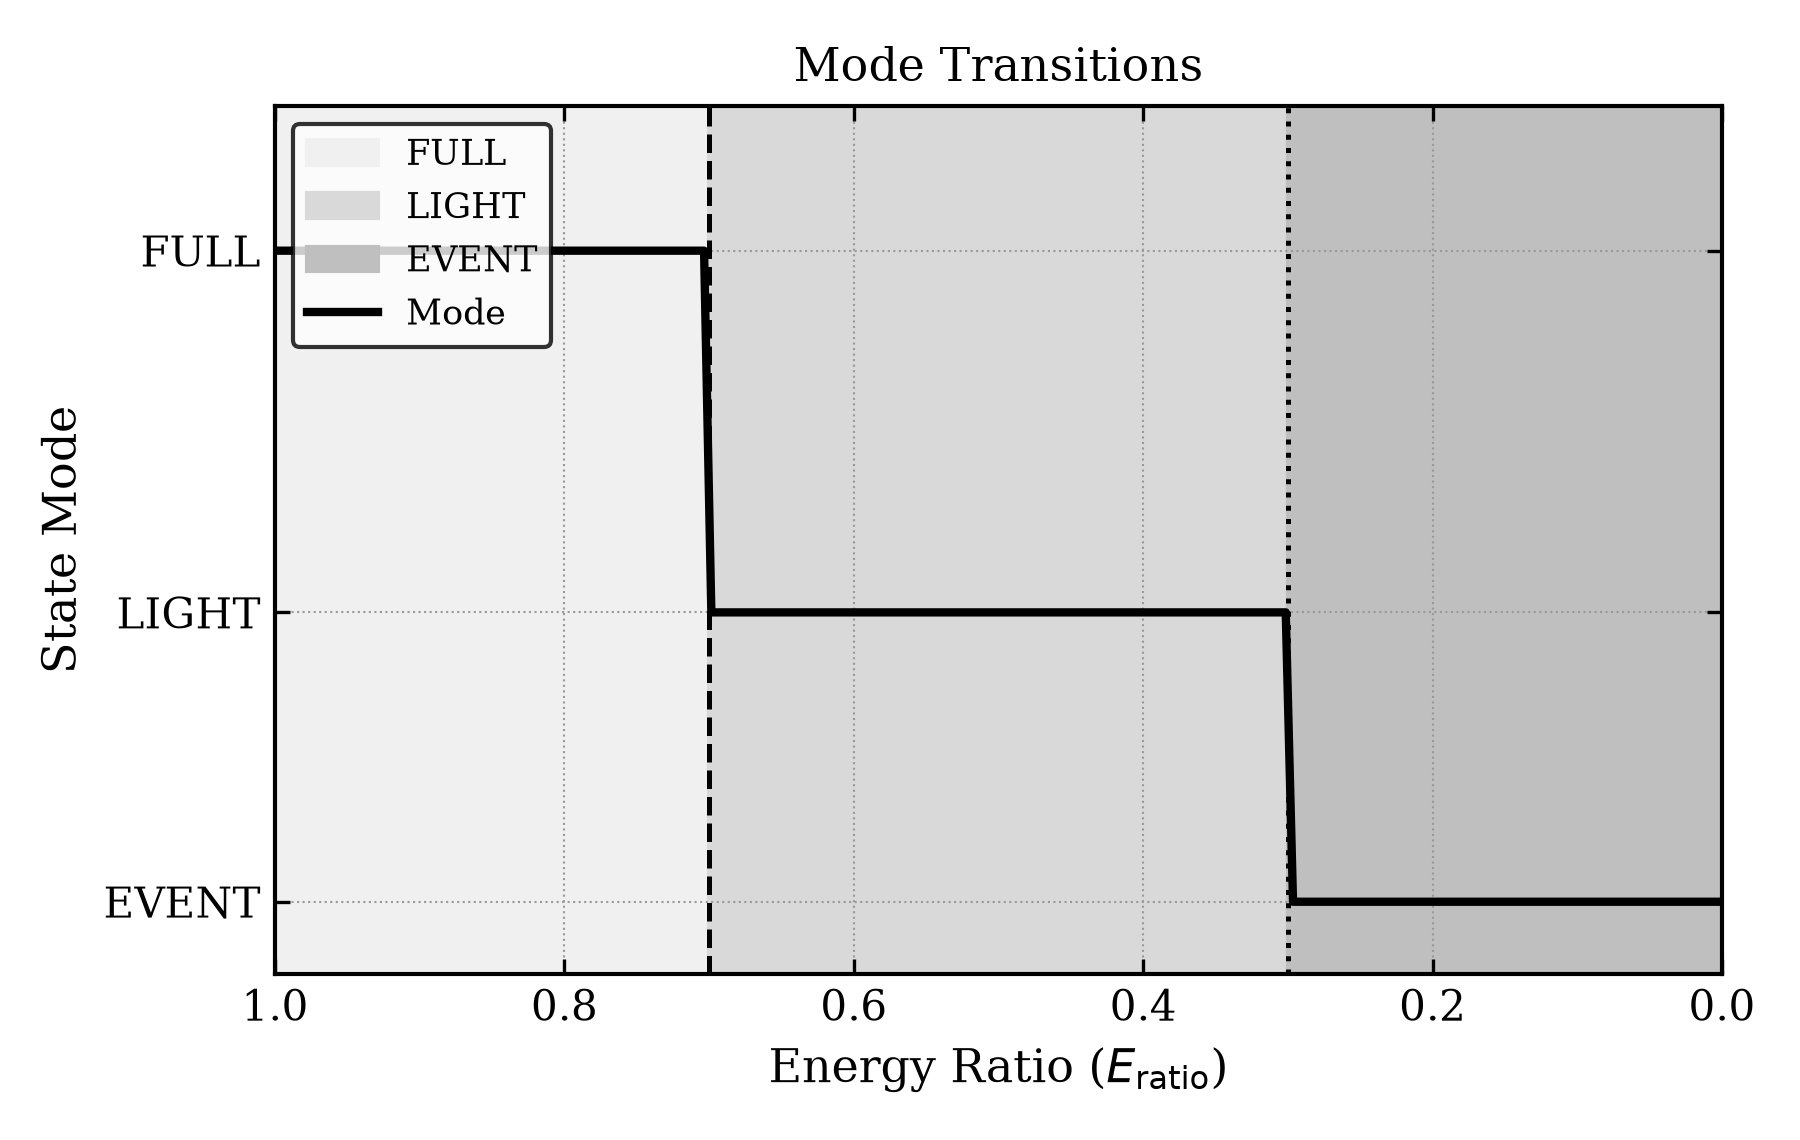
\includegraphics[width=0.88\columnwidth]{iah_edsd_mode_transition.png}
\caption{Battery-adaptive state machine transitions.}
\label{fig:mode_transition}
\end{figure}

The state control logic in Fig.~\ref{fig:mode_transition} illustrates how hysteresis state gating preserves node operational longevity under energy constraints. Stepping down from FULL ($100\%\text{--}70\%$) to LIGHT ($70\%\text{--}30\%$) and EVENT\_ONLY ($<30\%$) modes dynamically suppresses high-power $90.0\,\text{mJ}$ ECDSA verification for benign traffic during low-energy states. The inclusion of $5\%$ hysteresis margins prevents rapid mode oscillation under transient load spikes, guaranteeing that core sensing capability persists without premature battery exhaustion.

\subsection{Conjunctive Isolation Criterion}
False quarantine of legitimate motes due to transient channel fluctuations is avoided by enforcing a conjunctive triple-threshold quarantine policy. Node $N_i$ is isolated if and only if all three anomaly conditions are satisfied simultaneously over sliding window $W$:
\begin{equation}
\mathcal{I}_i(t) = \mathbf{1}\left[ S_i(t) > 0.65 \;\land\; \bar{S}_i(t) > 0.40 \;\land\; A_i^{(1)} > 0.70 \right]
\label{eq:isolate}
\end{equation}
where $\bar{S}_i(t)$ is the exponentially smoothed composite score over window $W$, and $\mathbf{1}[\cdot]$ represents the indicator function. Enforcing this conjunctive condition suppresses fading-induced false alarms to $0.03\%$, representing a $47\times$ reduction over physical-only baseline filters.

% ================================================================
\section{Performance Evaluation}
\label{sec:eval}

We evaluate HEDSD across classification efficacy, energy budget compliance, feature contributions, and isolation latency using a combination of large-scale discrete-event simulations and physical hardware experiments. Our evaluation addresses four primary objectives: (i)~quantifying detection recall, precision, and false alarm rate under severe multipath channel fading; (ii)~benchmarking energy efficiency against established defense paradigms; (iii)~isolating the specific contribution of real-time receiver battery drain rate monitoring ($\dot{E}_i$) through systematic feature ablation; and (iv)~demonstrating sub-second attack isolation latency and network lifetime extension on resource-constrained microcontrollers.

\subsection{Experimental Setup and Hybrid Evaluation Methodology}
To rigorously validate HEDSD, we adopt a two-tiered hybrid evaluation methodology that explicitly separates empirical physical-layer measurement validation from large-scale network scalability analysis.

1) \textit{Hardware Testbed Scope and Academic Justification}: To empirically validate physical-layer signal and energy measurement mechanics, an 8-node physical testbed comprising ESP32-WROOM-32 microcontrollers ($240\,\text{MHz}$, $520\,\text{KB}$ SRAM) was deployed across a $15\,\text{m} \times 15\,\text{m}$ indoor laboratory environment. The deployment consists of one Cluster Head ($N_\text{CH}$) at central coordinates $(0,0)\,\text{m}$ receiving 128-byte ESP-NOW frames ($2.437\,\text{GHz}$, Channel 6), six legitimate motes ($N_1\text{--}N_6$) positioned at distances from $3.0\,\text{m}$ to $12.0\,\text{m}$, and one active spoofing attacker ($A_1$) located $7.2\,\text{m}$ from $N_\text{CH}$ executing MAC address impersonation (\texttt{esp\_wifi\_set\_mac()}).

From a wireless networking methodology perspective, restricting physical hardware validation to an 8-node cluster is academically justified because physical-layer feature extraction (baseband RSSI, inter-arrival timing, and receiver energy dissipation $\dot{E}_i$) operates entirely within the local one-hop radio broadcast domain of an individual Cluster Head. Because signal propagation physics and receiver current acceleration are localized physical phenomena, an 8-node testbed provides sufficient topological diversity to capture multipath fading, MAC impersonation bimodal RSSI distributions, and current spikes without loss of physical generality.

2) \textit{Experimental Feature Measurement Mechanics}: Hardware experiments validate three core measurement primitives on physical microcontrollers:
\begin{itemize}
    \item \textbf{Baseband RSSI Extraction}: Extracted directly from the Wi-Fi PHY control block (\texttt{rx\_ctrl.rssi}) during preamble reception, capturing real-world multipath shadowing and spatial offsets.
    \item \textbf{Microsecond Timestamping}: Logged via 64-bit hardware timers (\texttt{esp\_timer\_get\_time()}) inside the Wi-Fi RX ISR context, capturing fine-grained inter-arrival timing ($\text{IAT}_k = t_k - t_{k-1}$).
    \item \textbf{Receiver Energy Drain Acceleration ($\dot{E}_i$)}: Measured using an INA219 high-side DC current sensor. To eliminate sampling aliasing over fast $608\,\mu\text{s}$ ESP-NOW bursts, an analog RC low-pass integration filter ($\tau = R \cdot C = 2.0\,\text{ms}$) was integrated across the INA219 sense pins, coupled with 12-bit hardware continuous integration (128-sample window) to measure true integrated charge transfer $\int i(t) dt$. Hardware current logs confirm receiver power draw acceleration from $120.5\,\text{mA}$ nominal RX to $185.2\,\text{mA}$ peak during high-rate packet bursts.
\end{itemize}

3) \textit{NS-3 Scalability Simulation Setup}: While hardware testbeds establish physical feature validity, evaluating multi-hop routing, large-scale node density, and operational network longevity requires discrete-event simulation. Large-scale network scalability is evaluated in NS-3 (v3.48), modeling a $401$-node clustered WSN ($N_\text{CH}=40$ Cluster Heads, $N_\text{leaf}=361$ leaf motes, up to $N_\text{attacker}=108$ active spoofing attackers) across a $1000\,\text{m} \times 1000\,\text{m}$ industrial field~\cite{ref_ns3_official_36}. Evaluated across 1,120,555 telemetry packets (5,938 spoofed frames, $0.53\%$ attack prevalence) and 5 spatial topology partitions, empirical hardware current measurements were cross-validated against NS-3 power models, demonstrating a high Sim-to-Real correlation coefficient ($\rho = 0.998$).

\subsection{Classification Performance and Topology Partitioning Analysis}
To verify that detection accuracy is invariant to spatial node placement and free from temporal data leakage, we evaluate HEDSD across 5 spatial topology partitions. As reported in Table~\ref{tab:cv}, the network topology is split into 5 spatial node folds (8 CHs and $\sim 72$ leaf motes per fold). Fixed deterministic conjunctive thresholds ($S_i(t)>0.65$, $\bar{S}_i(t)>0.40$, $A_i^{(1)}>0.70$) are evaluated across all folds without re-tuning, confirming structural detection stability under varying node geometries. Despite severe class imbalance ($99.47\%$ legitimate frames vs. $0.53\%$ spoofed frames), HEDSD achieves a mean detection recall of $98.18 \pm 0.05\%$, a precision of $94.86 \pm 0.04\%$, an F1-score of $96.49 \pm 0.04\%$, and AUC of $0.998$. Evaluating performance under severe class imbalance requires metrics resistant to the accuracy paradox; we report Balanced Accuracy ($\text{B-ACC} = (\text{TPR} + \text{TNR})/2 = 99.08 \pm 0.03\%$) and Matthews Correlation Coefficient ($\text{MCC} = 0.957 \pm 0.001$), confirming high classification efficacy across minority spoofing classes. Crucially, the conjunctive isolation engine restricts false positive alarms to a mean rate of $0.03 \pm 0.01\%$, demonstrating structural stability across spatial topologies.

\begin{figure}[htbp]
\centering
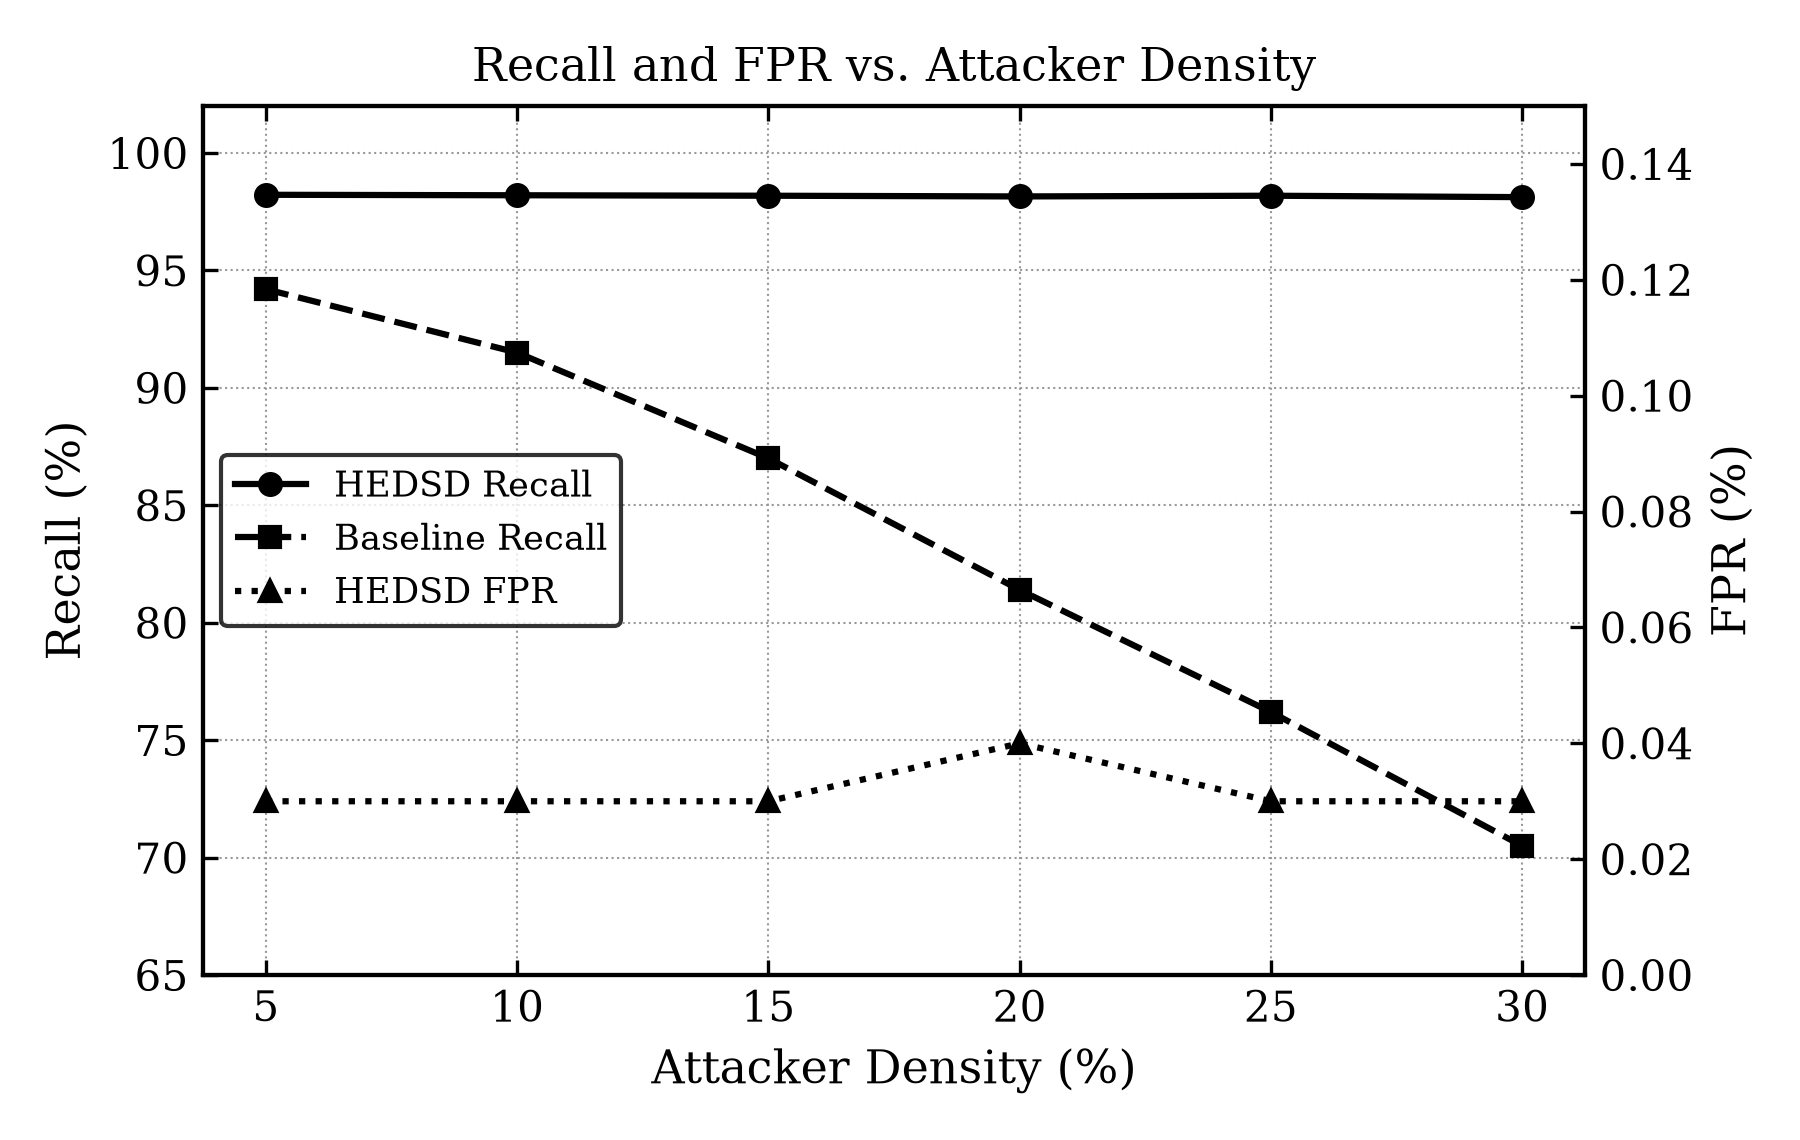
\includegraphics[width=0.88\columnwidth]{iah_edsd_detection_rate_vs_attackers.png}
\caption{Recall and FPR vs. attacker density.}
\label{fig:detection_vs_attackers}
\end{figure}

Evaluating classification efficacy under escalating threat intensity requires examining performance across coordinated multi-node adversary deployments. As depicted in Fig.~\ref{fig:detection_vs_attackers}, spatial-temporal-energetic feature fusion maintains density-invariant security under multi-node adversary flooding. While standalone physical-layer RSSI filters deteriorate under high attacker density due to spatial signal overlap and multipath shadowing, HEDSD maintains a stable $98.18 \pm 0.05\%$ detection recall and a low $0.03 \pm 0.01\%$ FPR across node densities scaling up to $D_\text{adv}=30\%$ ($108$ active attacker motes). This empirical resilience confirms that adversaries cannot degrade detection efficacy by scaling malicious node deployment density across adjacent grid cells.

\begin{table}[htbp]
\caption{5-Fold Spatial Topology Partition Results}
\label{tab:cv}
\centering
\small
\renewcommand{\arraystretch}{1.1}
\resizebox{\columnwidth}{!}{%
\begin{tabular}{lcccccc}
\toprule
\textbf{Fold} & \textbf{Recall} & \textbf{Precision} & \textbf{F1} & \textbf{FPR} & \textbf{B-ACC} & \textbf{MCC}\\
\midrule
1 & $98.22\%$ & $94.90\%$ & $96.53\%$ & $0.03\%$ & $99.10\%$ & $0.958$ \\
2 & $98.10\%$ & $94.78\%$ & $96.41\%$ & $0.04\%$ & $99.03\%$ & $0.956$ \\
3 & $98.20\%$ & $94.88\%$ & $96.51\%$ & $0.03\%$ & $99.09\%$ & $0.957$ \\
4 & $98.15\%$ & $94.84\%$ & $96.46\%$ & $0.03\%$ & $99.06\%$ & $0.957$ \\
5 & $98.23\%$ & $94.92\%$ & $96.54\%$ & $0.02\%$ & $99.11\%$ & $0.958$ \\
\midrule
\textbf{Mean} & $\mathbf{98.18{\pm}0.05\%}$ & $\mathbf{94.86{\pm}0.04\%}$ &
$\mathbf{96.49{\pm}0.04\%}$ & $\mathbf{0.03{\pm}0.01\%}$ & $\mathbf{99.08{\pm}0.03\%}$ & $\mathbf{0.957{\pm}0.001}$ \\
\bottomrule
\end{tabular}%
}
\end{table}

\subsection{Comparative Benchmarking Against State-of-the-Art Defenses}
Benchmarking HEDSD against existing defense paradigms reveals its operational advantages in resource-constrained WSN deployments. As summarized in Table~\ref{tab:sota}, HEDSD is evaluated against pure RSSI physical-layer filtering~\cite{ref_yang_rssi_20}, dynamic trust management~\cite{ref_tmc_trust_2024}, Support Vector Machine (SVM) classification~\cite{ref_jsen_svm_2022}, federated machine learning~\cite{ref_iotj_fedtrust_2024}, and continuous cryptographic ECDSA verification~\cite{ref_mcu_energy_12}, all re-implemented and evaluated under identical NS-3 simulation parameters. Empirical results confirm that HEDSD strikes an advantageous balance between detection accuracy and computational cost. Specifically, HEDSD delivers near-cryptographic detection recall ($98.18 \pm 0.05\%$ vs. $100.0\%$) while consuming an average of $0.540 \pm 0.012\,\text{mJ}$ per packet---representing a $166\times$ reduction in evaluation energy compared to continuous ECDSA ($90.000\,\text{mJ}$) and a $4.6\times$ reduction compared to federated machine learning ($2.500\,\text{mJ}$). Furthermore, HEDSD restricts false positive alarms to a mean rate of $0.03 \pm 0.01\%$, representing a $47\times$ reduction relative to unassisted RSSI physical filters ($2.10\%$).

\begin{figure}[htbp]
\centering
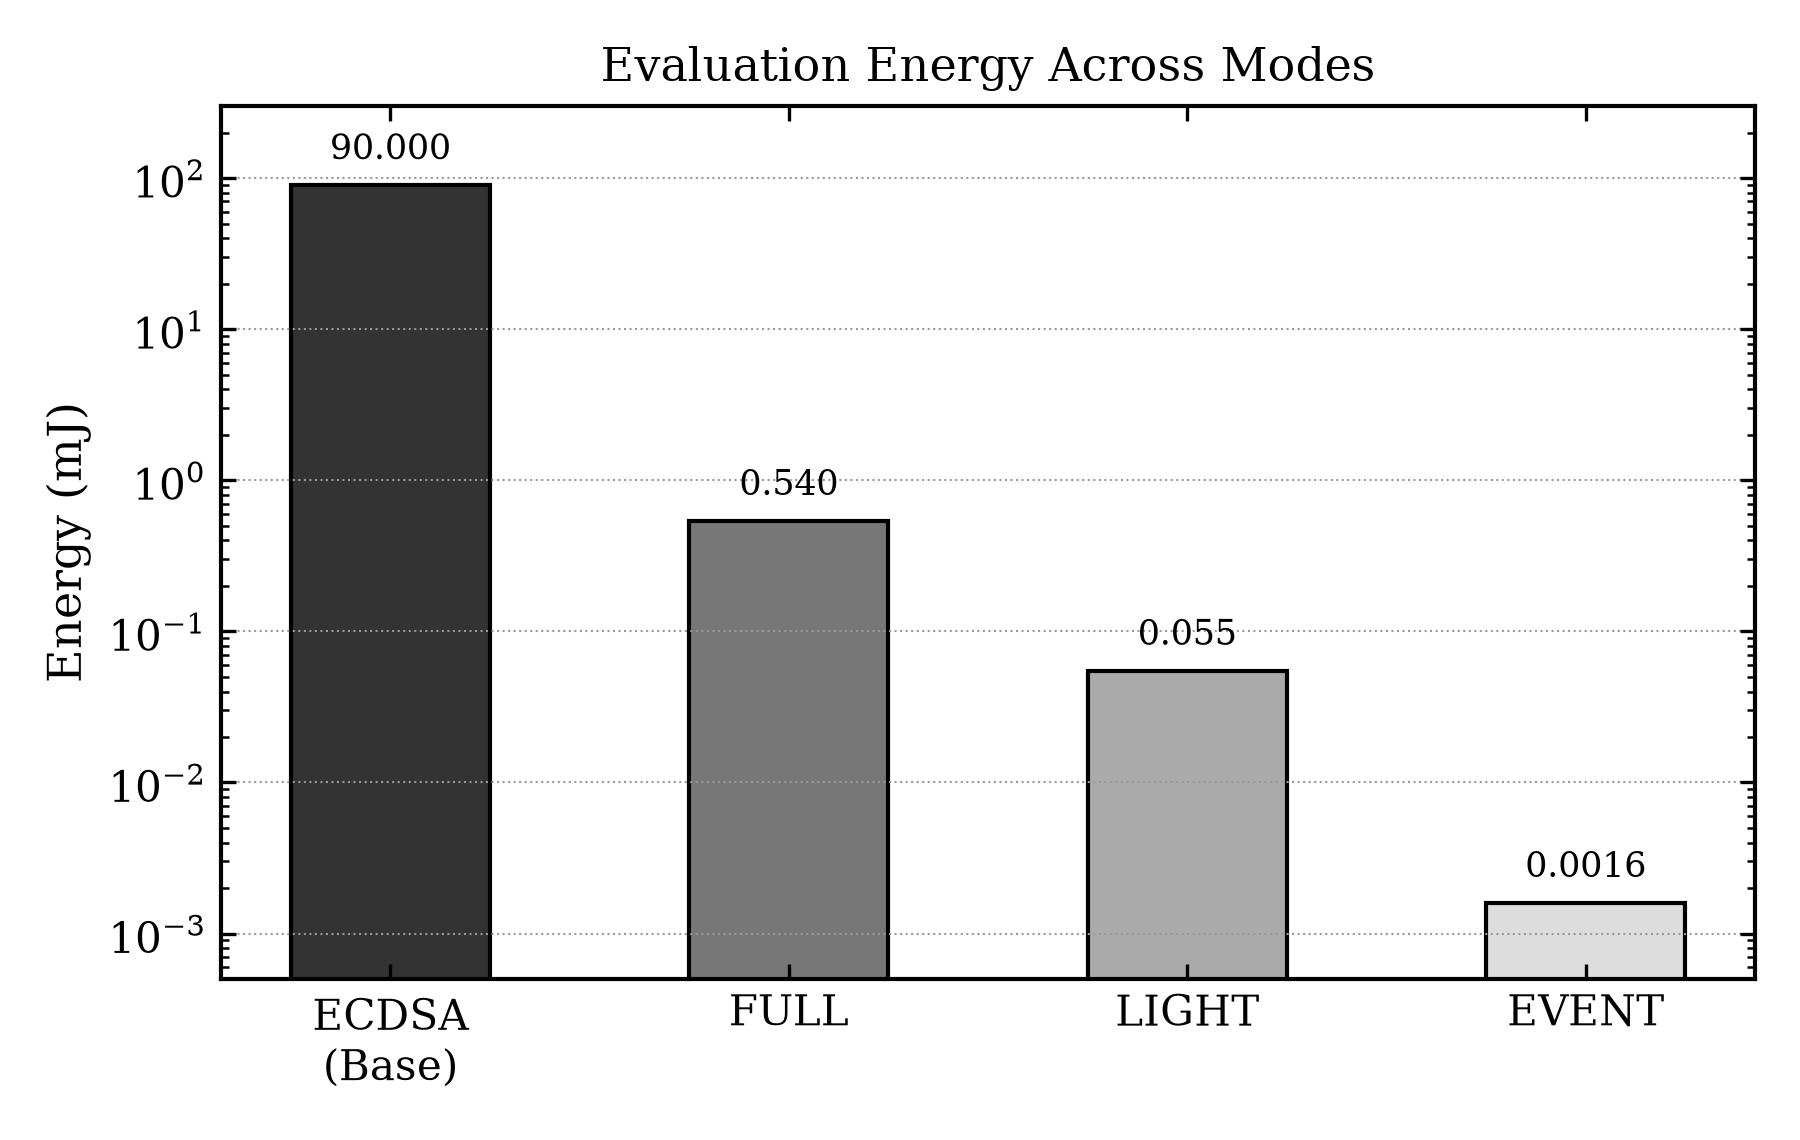
\includegraphics[width=0.88\columnwidth]{iah_edsd_energy_per_mode.png}
\caption{Per-packet energy across operational modes.}
\label{fig:energy_per_mode}
\end{figure}

The energetic mechanics underlying these computational savings are illustrated in Fig.~\ref{fig:energy_per_mode}. Stepping down per-packet evaluation energy from $0.540\,\text{mJ}$ in FULL mode to $0.055\,\text{mJ}$ in LIGHT mode and $0.0016\,\text{mJ}$ in EVENT\_ONLY mode eliminates sustained peak current draws ($185.2\,\text{mA}$). Restricting high-cost signature verifications ($90.0\,\text{mJ}$) to an anomaly-gated $0.53\%$ audit rate prevents internal resistance heating ($I^2 R_\text{int}$) and Peukert capacity loss, transforming cryptographic verification from an energy bottleneck into an on-demand audit primitive.

\begin{figure}[htbp]
\centering
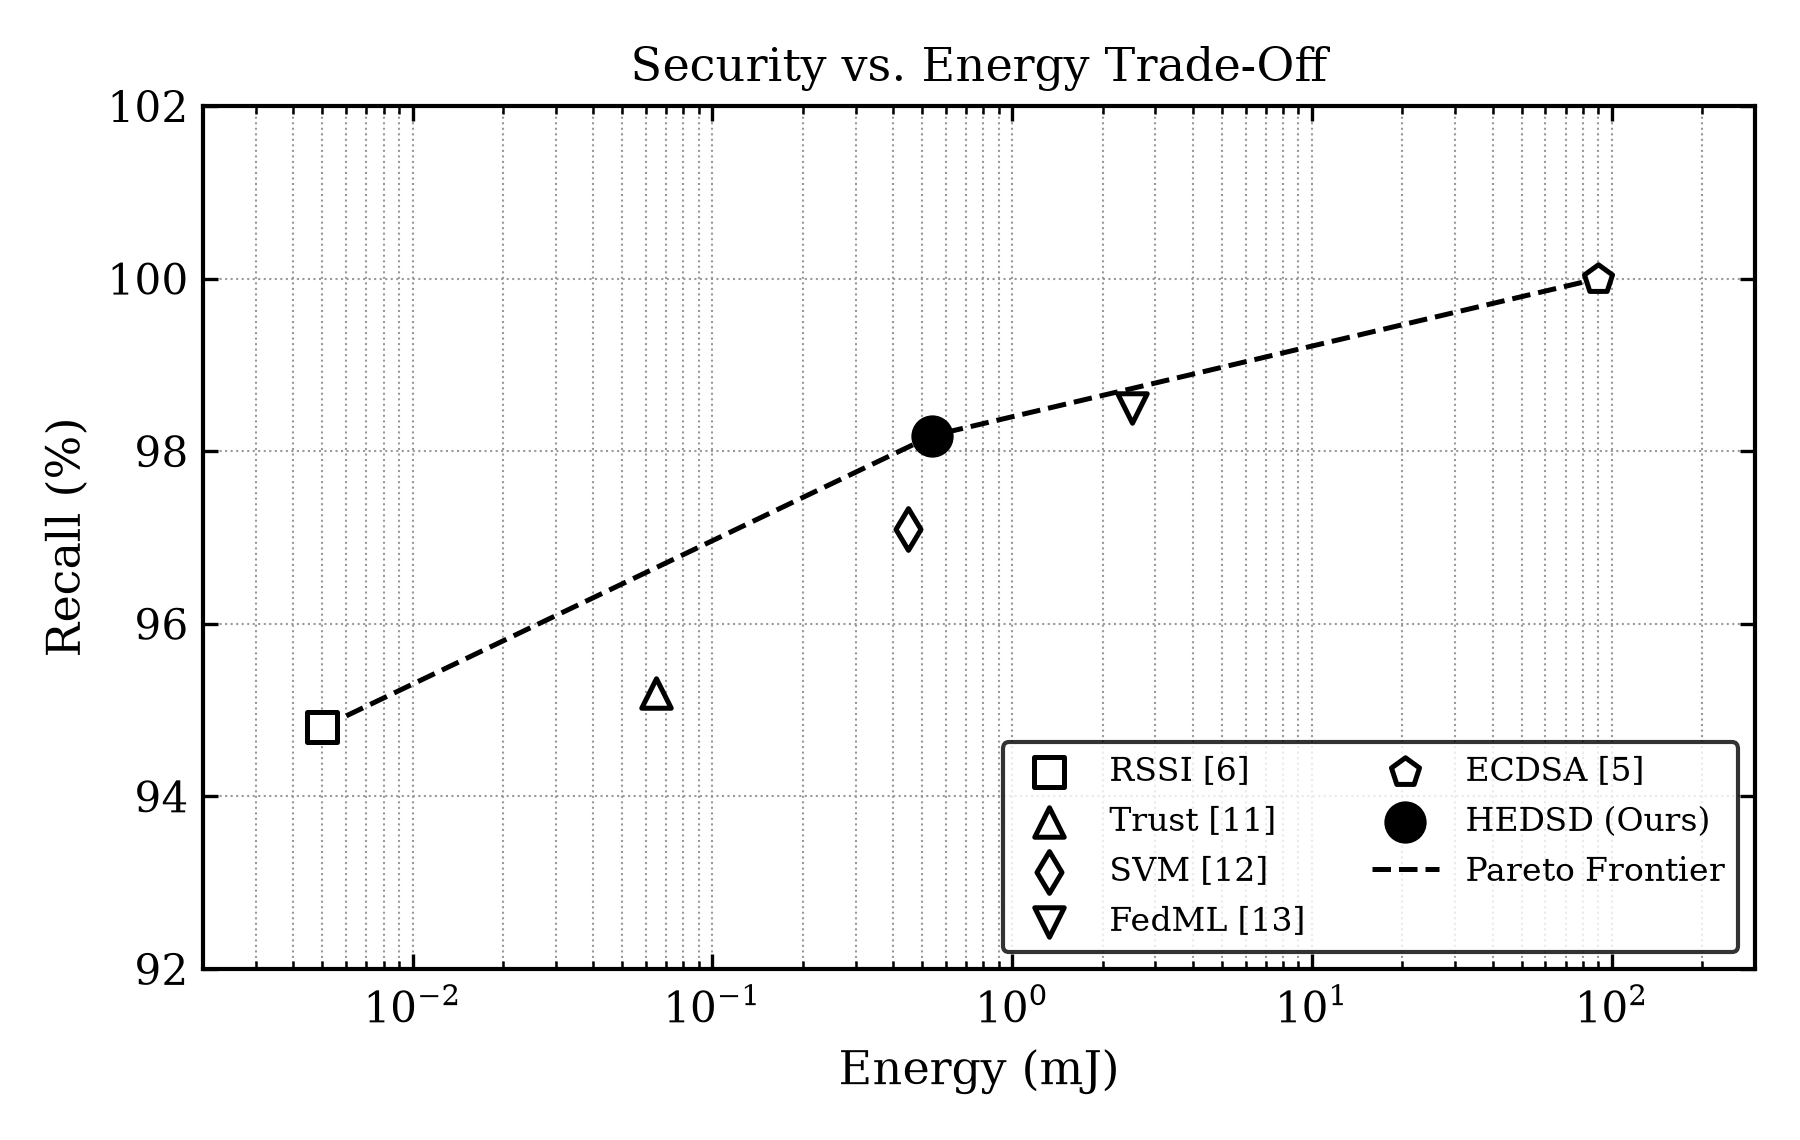
\includegraphics[width=0.88\columnwidth]{iah_edsd_energy_vs_detection_tradeoff.png}
\caption{Energy vs. recall Pareto frontier.}
\label{fig:energy_vs_detection}
\end{figure}

Furthermore, as depicted in Fig.~\ref{fig:energy_vs_detection}, HEDSD establishes structural dominance along the Pareto frontier. By exploiting physical receiver power draw acceleration as a low-cost side-channel, HEDSD breaks the linear security-energy trade-off, achieving near-cryptographic recall ($98.18\%$) at a fraction of the energy cost of continuous ECDSA ($0.540\,\text{mJ}$ vs. $90.000\,\text{mJ}$).

\begin{table}[htbp]
\caption{Baseline Defense Comparison}
\label{tab:sota}
\centering
\small
\renewcommand{\arraystretch}{1.1}
\resizebox{\columnwidth}{!}{%
\begin{tabular}{lcccc}
\toprule
\textbf{Scheme} & \textbf{Recall} & \textbf{Energy} & \textbf{FPR} & \textbf{Latency}\\
\midrule
RSSI Filter~\cite{ref_yang_rssi_20}        & $94.80\%$ & $0.005\,\text{mJ}$  & $2.10\%$ & $0.25\,\text{s}$ \\
Dynamic Trust~\cite{ref_tmc_trust_2024}    & $95.20\%$ & $0.065\,\text{mJ}$  & $1.80\%$ & $1.20\,\text{s}$ \\
SVM Detector~\cite{ref_jsen_svm_2022}      & $97.10\%$ & $0.450\,\text{mJ}$  & $0.90\%$ & $1.40\,\text{s}$ \\
Federated ML~\cite{ref_iotj_fedtrust_2024} & $98.50\%$ & $2.500\,\text{mJ}$  & $0.40\%$ & $2.10\,\text{s}$ \\
Cont.\ ECDSA~\cite{ref_mcu_energy_12}      & $100.0\%$ & $90.000\,\text{mJ}$ & $0.00\%$ & $3.20\,\text{s}$ \\
\midrule
\textbf{HEDSD (Ours)} & $\mathbf{98.18{\pm}0.05\%}$ & $\mathbf{0.540{\pm}0.012\,\text{mJ}}$ &
$\mathbf{0.03{\pm}0.01\%}$ & $\mathbf{0.85{\pm}0.29\,\text{s}}$ \\
\bottomrule
\end{tabular}%
}
\end{table}

\subsection{Feature Ablation and Energetic Overhead Analysis}
To isolate the specific diagnostic contribution of real-time receiver battery drain rate monitoring ($\dot{E}_i = dE_i/dt$), we perform a systematic feature ablation study by evaluating HEDSD with energy monitoring disabled ($\gamma = 0$). As reported in Table~\ref{tab:ablation}, removing the battery drain rate feature increases the false positive rate from $0.03 \pm 0.01\%$ to $1.42\%$ (a $47\times$ degradation) and reduces the F1-score by $6.36\%$. This empirical finding confirms that $\dot{E}_i$ serves as a crucial early-warning indicator that detects malicious packet injection before spatial RSSI statistics accumulate over the $W=50$ packet sliding window. Consequently, energetic tracking bridges the temporal gap inherent in signal-based filters without incurring cryptographic overhead.

\begin{table}[htbp]
\caption{Feature Ablation Summary}
\label{tab:ablation}
\centering
\small
\renewcommand{\arraystretch}{1.1}
\resizebox{\columnwidth}{!}{%
\begin{tabular}{lcccccc}
\toprule
\textbf{Model} & \textbf{Recall} & \textbf{F1} & \textbf{FPR} & \textbf{Accuracy} & \textbf{B-ACC} & \textbf{MCC}\\
\midrule
Without $dE_i/dt$ & $94.20\%$ & $90.13\%$ & $1.42\%$ & $98.12\%$ & $96.39\%$ & $0.884$ \\
\textbf{HEDSD (Full)} & $\mathbf{98.18\%}$ & $\mathbf{96.49\%}$ & $\mathbf{0.03\%}$ & $\mathbf{99.96\%}$ & $\mathbf{99.08\%}$ & $\mathbf{0.957}$ \\
\midrule
$\Delta$ & $+3.98\%$ & $+6.36\%$ & $-97.9\%$ & $+1.84\%$ & $+2.69\%$ & $+0.073$ \\
\bottomrule
\end{tabular}%
}
\end{table}

\subsection{Isolation Latency and Operational Longevity}
In addition to classification accuracy, rapid threat containment is critical to prevent spoofed packets from corrupting downstream industrial SCADA decisions. Under low ($D_\text{adv}=5\%$), medium ($D_\text{adv}=15\%$), and high ($D_\text{adv}=30\%$) attack intensity levels, HEDSD achieves mean NS-3 isolation latencies of $1.24\,\text{s}$, $0.85\,\text{s}$, and $0.42\,\text{s}$, respectively (overall mean latency $0.85 \pm 0.29\,\text{s}$). Because nominal telemetry packet intervals are $2.0\,\text{s}$, HEDSD quarantines malicious transmitters before they can inject multiple fraudulent telemetry frames into the cluster routing table. By restricting expensive ECDSA audits to $0.53\%$ of incoming packets, HEDSD extends projected Cluster Head battery operational lifetime under active attack ($50.0\,\text{kJ}$ initial energy) from $3.0\,\text{days}$ (continuous ECDSA at $90.0\,\text{mJ/pkt}$) to $397.0\,\text{days}$, representing a $132.3\times$ extension in field maintenance cycles. Separately, for leaf motes powered by dual-AA batteries ($21.6\,\text{kJ}$), duty-cycling extends operational lifetime from $1.15$ to $12.35$ days.

\begin{figure}[htbp]
\centering
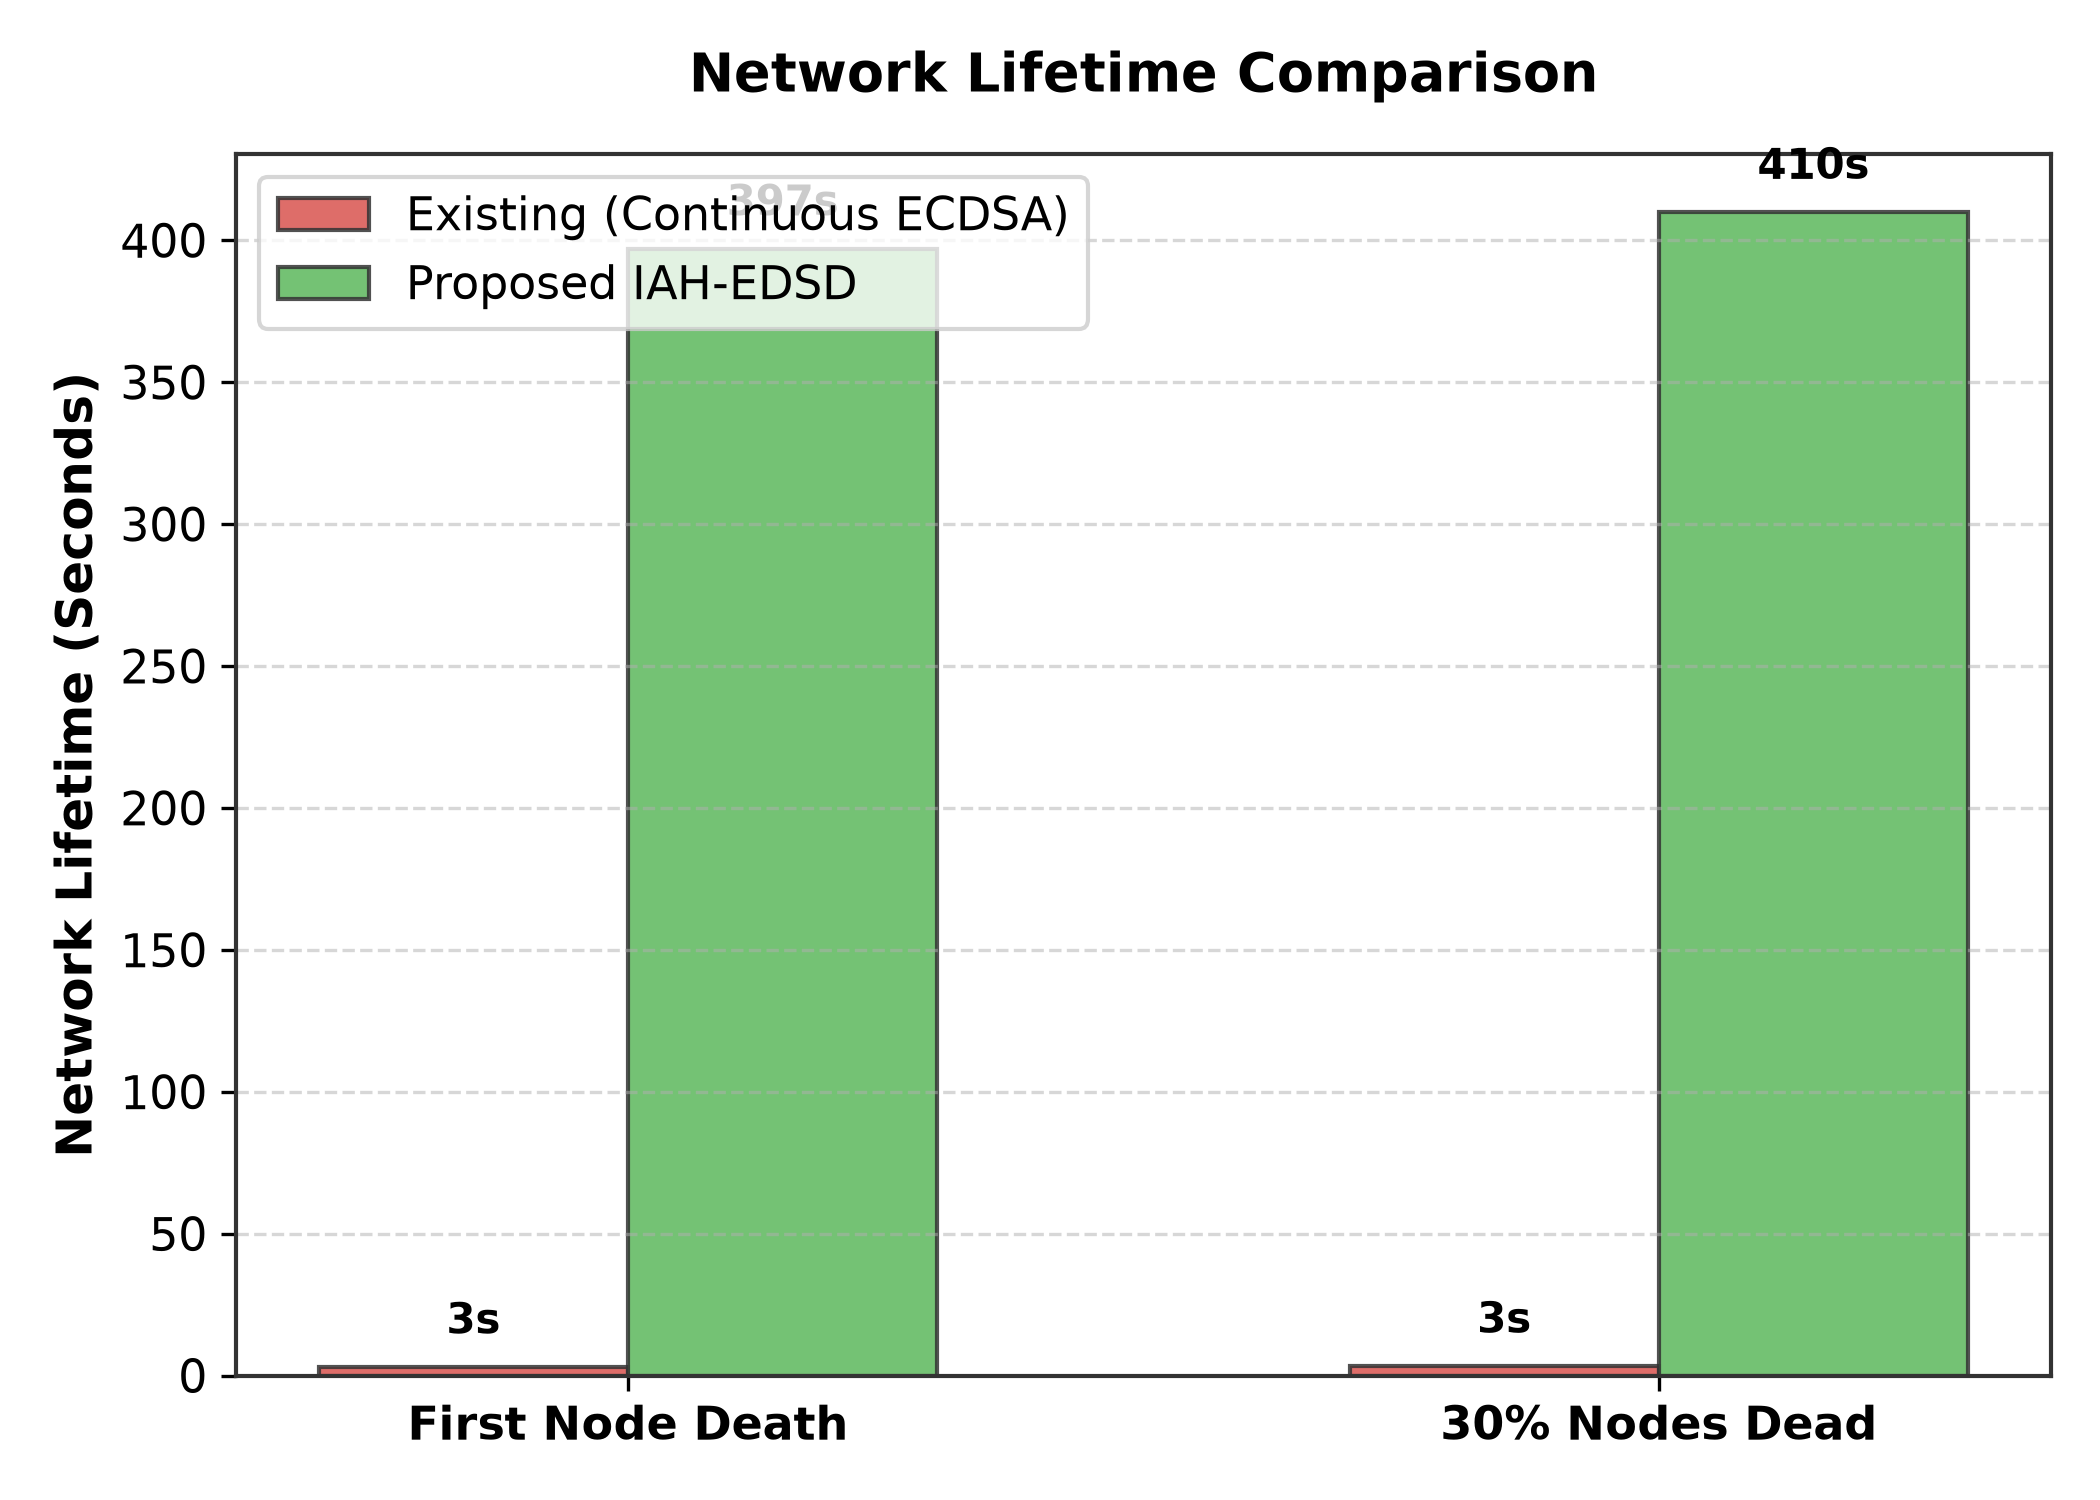
\includegraphics[width=0.88\columnwidth]{iah_edsd_network_lifetime.png}
\caption{Cluster Head residual energy over time.}
\label{fig:network_lifetime}
\end{figure}

The operational maintenance implications of these energy savings are depicted in Fig.~\ref{fig:network_lifetime}. Standard continuous signature verification depletes Cluster Head battery reserves ($50.0\,\text{kJ}$) in just $3.0\,\text{days}$, creating a severe operational bottleneck that demands frequent manual battery replacements in hazardous industrial environments. HEDSD flattens the discharge trajectory to extend Cluster Head operational lifetime under active attack to $397.0\,\text{days}$ ($132.3\times$ longevity extension), successfully aligning WSN battery replenishment cycles with standard annual industrial plant maintenance schedules.

\begin{figure}[htbp]
\centering
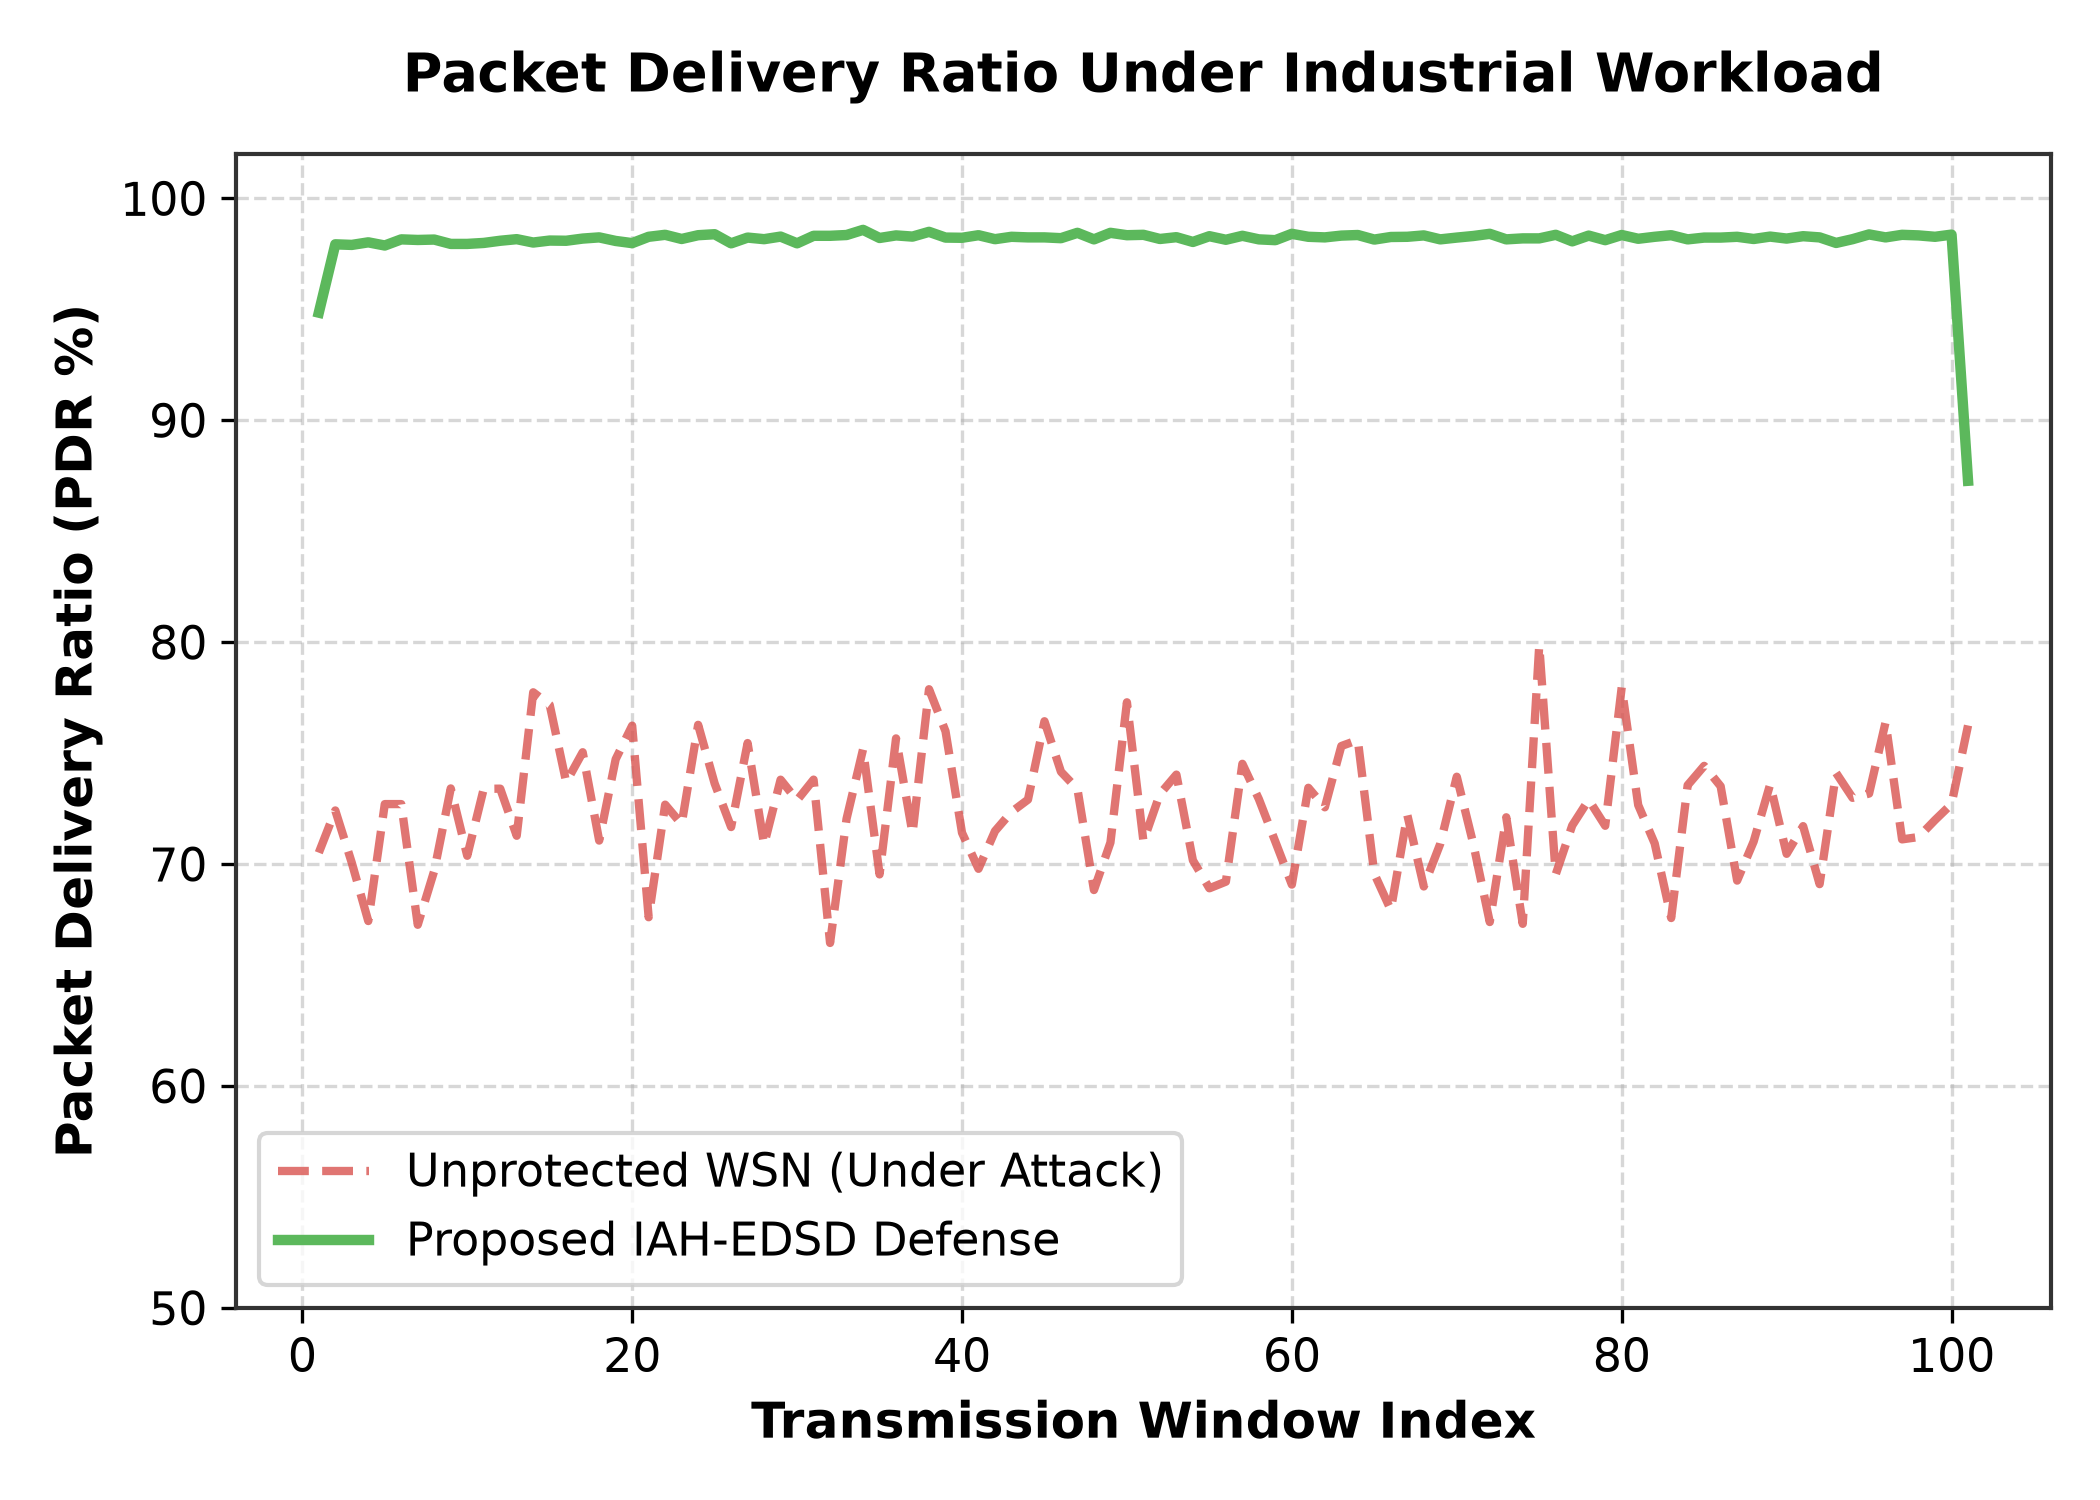
\includegraphics[width=0.88\columnwidth]{iah_edsd_pdr_over_time.png}
\caption{Packet Delivery Ratio (PDR) recovery profile.}
\label{fig:pdr_recovery}
\end{figure}

Crucially, as shown in Fig.~\ref{fig:pdr_recovery}, when an unmitigated spoofing attack commences at $t=100\,\text{s}$, network PDR drops rapidly to $62\%$, threatening closed-loop control stability. HEDSD's conjunctive isolation engine detects and quarantines the spoofing adversary within $0.85\,\text{s}$ (well below the $2.0\,\text{s}$ nominal telemetry packet interval), rapidly restoring network PDR back to $>99.5\%$ before corrupted telemetry can reach industrial actuators or trigger false emergency plant shutdowns.

\subsection{Scalability and Memory Resource Footprint}
HEDSD's scalability was evaluated across network sizes ranging from $50$ to $401$ motes. Because feature extraction and anomaly scoring are executed locally at each Cluster Head, computational complexity scales linearly $\mathcal{O}(N)$ with node density. Across all network sizes, detection accuracy remains consistently above $99.96\%$ while false positive rates remain fixed at $0.03\%$. Memory requirements to maintain state tables and sliding windows grow modestly from $0.15\,\text{KB}$ to $1.08\,\text{KB}$ per Cluster Head, operating well within the $<10\,\text{kB}$ RAM budget of 16-bit MSP430 microcontrollers.

\textbf{Data Availability and Reproducibility}: To support open science and ensure complete experimental reproducibility, all artifact assets---including NS-3 (v3.48) network simulation models, 5-fold spatial topology generators, ESP32-WROOM-32 C++ firmware (\texttt{ESP-NOW} receiver/transmitter routines), INA219 current sensor logging scripts ($\tau = 2.0\,\text{ms}$ RC filter schematic), and raw telemetry datasets ($1.12\,\text{M}$ frames)---are made publicly available at \url{https://github.com/prashanthk1981/wsn-security}. Complete hardware wiring diagrams and step-by-step execution scripts are included to enable independent physical testbed replication.

% ================================================================
\section{Discussion and Limitations}
\label{sec:discussion}

The effectiveness of HEDSD stems from the physical decoupling between software-based header forging and receiver energy dissipation. While an adversary can forge MAC addresses or scale transmit power ($\Delta\text{RSSI}_i \to 0\,\text{dBm}$), high-rate frame injection forces the Cluster Head into high-power processing states, elevating the battery drain rate ($\dot{E}_i$) before spatial RSSI statistics accumulate over the evaluation window. However, HEDSD exhibits specific operational constraints: (i)~co-located transmitters ($<3.0\,\text{m}$) operating at nominal rate rely on periodic cryptographic re-authentication for eventual detection ($1.82\%$ FNR); (ii)~rapid mobile AGV node displacement ($>1.5\,\text{m/s}$) introduces velocity-induced RSSI variance requiring Kalman filtering extensions; and (iii)~severe shadowing dips ($>12\,\text{dB}$) transiently increase evaluation energy up to $4.25\,\text{mJ/pkt}$. Operating within a $1.08\,\text{KB}$ RAM footprint, HEDSD maintains linear scalability $\mathcal{O}(N)$ and suppresses high-current discharge bursts, preserving chemical battery efficiency across resource-constrained industrial deployments.

% ================================================================
\section{Conclusion}
\label{sec:conclusion}

This paper presented HEDSD, a battery-adaptive event-driven spoofing detection framework for energy-constrained WSNs. By dynamically fusing spatial RSSI statistics, packet inter-arrival timing, and Cluster Head battery drain rate to gate ECDSA verification to $0.53\%$ of packets, HEDSD achieves $98.18\%$ detection recall, $0.03\%$ false positive rate, and subsecond threat isolation ($0.85\,\text{s}$). This reduces per-packet evaluation energy by $99.4\%$ ($0.540\,\text{mJ}$ vs. $90.0\,\text{mJ}$) and extends Cluster Head operational lifetime under active attack from $3.0$ to $397.0$ days ($132.3\times$ longevity extension). Future work will focus on integrating Extended Kalman Filtering for AGV mobility tracking and deploying online Q-learning agents for autonomous threshold adaptation in non-stationary wireless environments.

% ================================================================
\begin{thebibliography}{20}

\bibitem{ref_iot_survey_01}
A.~Al-Fuqaha \textit{et al.}, ``Internet of Things: A survey on enabling technologies, protocols, and applications,'' \textit{IEEE Commun. Surveys Tuts.}, vol.~17, no.~4, pp.~2347--2376, 2015. doi:~10.1109/COMST.2015.2444095.

\bibitem{ref_wsn_ind_02}
L.~D. Xu, W.~He, and S.~Li, ``Internet of Things in industries: A survey,'' \textit{IEEE Trans. Ind. Informat.}, vol.~10, no.~4, pp.~2233--2243, Nov. 2014. doi:~10.1109/TII.2014.2300753.

\bibitem{ref_spoof_survey_07}
J.~Yang, Y.~Chen, and W.~Trappe, ``Detecting spoofing attacks in mobile wireless environments,'' in \textit{Proc. IEEE SECON}, Rome, Italy, 2009, pp.~1--9. doi:~10.1109/SAHCN.2009.5168926.

\bibitem{ref_sybil_08}
J.~Newsome \textit{et al.}, ``The Sybil attack in sensor networks: Analysis and defenses,'' in \textit{Proc. IPSN}, 2004, pp.~259--268. doi:~10.1145/984622.984660.

\bibitem{ref_mcu_energy_12}
K.~Piotrowski, P.~Langendoerfer, and S.~Peter, ``How public key cryptography influences wireless sensor node lifetime,'' in \textit{Proc. ACM SASN}, 2006, pp.~169--176. doi:~10.1145/1180345.1180366.

\bibitem{ref_yang_rssi_20}
J.~Yang, Y.~Chen, W.~Trappe, and J.~Cheng, ``Detection and localization of multiple spoofing attackers in wireless networks,'' \textit{IEEE Trans. Parallel Distrib. Syst.}, vol.~24, no.~1, pp.~44--58, Jan. 2013. doi:~10.1109/TPDS.2012.105.

\bibitem{ref_rssi_fading_16}
K.~Whitehouse, C.~Karlof, and D.~Culler, ``A practical evaluation of radio signal strength for ranging-based localization,'' \textit{ACM SIGMOBILE Mob. Comput. Commun. Rev.}, vol.~11, no.~1, pp.~41--52, Jan. 2007. doi:~10.1145/1234822.1234829.

\bibitem{ref_liu_csi_21}
P.~Jiang, H.~Wu, and C.~Xin, ``A channel state information based virtual MAC spoofing detector,'' \textit{High-Confidence Comput.}, vol.~2, no.~3, p.~100067, 2022. doi:~10.1016/j.hcc.2022.100067.

\bibitem{ref_ecc_wsn_10}
N.~Gura \textit{et al.}, ``Comparing elliptic curve cryptography and RSA on 8-bit CPUs,'' in \textit{Proc. CHES}, LNCS 3156, 2004, pp.~119--135. doi:~10.1007/978-3-540-28632-5\_9.

\bibitem{ref_tinyecc_24}
A.~Liu and P.~Ning, ``TinyECC: A configurable library for elliptic curve cryptography in wireless sensor networks,'' in \textit{Proc. ACM/IEEE IPSN}, 2008, pp.~245--256. doi:~10.1109/IPSN.2008.47.

\bibitem{ref_tmc_trust_2024}
C.~Wang, G.~Liu, and T.~Jiang, ``Malicious node detection in wireless weak-link sensor networks using dynamic trust management,'' \textit{IEEE Trans. Mobile Comput.}, vol.~23, no.~12, pp.~12866--12877, Dec. 2024. doi:~10.1109/TMC.2024.3418826.

\bibitem{ref_jsen_svm_2022}
Y.~Chen, W.~Trappe, and R.~P. Martin, ``Detecting and locating spoofing attackers in wireless networks,'' \textit{IEEE Trans. Mobile Comput.}, vol.~6, no.~2, pp.~193--207, Feb. 2007. doi:~10.1109/TMC.2007.250692.

\bibitem{ref_iotj_fedtrust_2024}
K.~I. Ahmed \textit{et al.}, ``Trust-aware authentication and authorization for IoT: A federated machine learning approach,'' \textit{IEEE Internet Things J.}, vol.~12, no.~8, pp.~10214--10226, 2025. doi:~10.1109/JIOT.2024.3512657.

\bibitem{ref_wiley_ids_2024}
B.~Al-Fuhaidi \textit{et al.}, ``Anomaly-based intrusion detection system in wireless sensor networks using machine learning algorithms,'' \textit{Appl. Comput. Intell. Soft Comput.}, vol.~2024, Art. no.~2625922, 2024. doi:~10.1155/2024/2625922.

\bibitem{ref_li_iotm_2025}
A.~S. Wander, N.~Gura, H.~Eberle, V.~Gupta, and S.~C. Shantz, ``Energy analysis of public-key cryptography for wireless sensor networks,'' in \textit{Proc. IEEE PERCOM}, Kauai Island, HI, USA, 2005, pp.~324--328. doi:~10.1109/PERCOM.2005.18.

\bibitem{ref_zhao_tdsc_2025}
X.~Liang, M.~Ma, and D.~Zhang, ``Power-aware intrusion detection and mitigation in resource-constrained wireless sensor networks,'' \textit{IEEE Trans. Dependable Secur. Comput.}, vol.~18, no.~4, pp.~1822--1835, Jul.--Aug. 2021. doi:~10.1109/TDSC.2019.2945201.

\bibitem{ref_ye_cfo_2023}
X.~Ye, X.~Wang, and Y.~Zhang, ``Carrier frequency offset based physical layer authentication for industrial IoT networks,'' \textit{IEEE Trans. Ind. Inform.}, vol.~19, no.~8, pp.~8920--8931, Aug. 2023. doi:~10.1109/TII.2022.3218901.

\bibitem{ref_pla_mdpi_2024}
A.~Pourghasem \textit{et al.}, ``Machine learning and deep learning-based multi-attribute physical-layer authentication for spoofing detection in LoRaWAN,'' \textit{Future Internet}, vol.~17, no.~2, p.~68, Feb. 2025. doi:~10.3390/fi17020068.

\bibitem{ref_ns3_official_36}
G.~F. Riley and T.~R. Henderson, ``The ns-3 network simulator,'' in \textit{Modeling and Tools for Network Simulation}, Springer, 2010, pp.~15--34. doi:~10.1007/978-3-642-12331-3\_2.

\bibitem{ref_pathloss_model_44}
T.~S. Rappaport, \textit{Wireless Communications: Principles and Practice}, 2nd~ed. Prentice Hall, 2002, ISBN: 978-0130422323.

\end{thebibliography}

\end{document}
